% !TEX root = sum1.tex
\section{Results}
We carried out several experiments, including comparing the running time of decomposition and Integer programming, comparing the number of people served using the feasible seat planning and Integer programming methods, analyzing different policies under the two booking situations, evaluating the results under varying demands, assessing the results for different numbers of people in each period and finally investigating the impact of seat layout on the number of served people.


\subsection{Running time of Benders Decomposition and IP}\label{Bender_IP}
% At first, we compare the running time of these two methods. 

The running times of solving DEF directly and solving the relaxation of DEF with Benders decomposition are shown in Table \ref{tab_1}.

\begin{table}[ht]
  \centering
  \caption{Running time of Decomposion and IP}\label{tab_1}
  \begin{tabular}{|l|l|l|l|l|l|l|}
  \hline
  \# of scenarios & demands & running time of IP(s) & Benders (s) & \# of rows & \# of groups & \# of seats\\
  \hline
  1000  & (150, 350) & 5.1  & 0.13 & 30 & 8 & (21, 50)\\
  5000  & & 28.73 & 0.47 & 30 & 8 \\
  10000 & & 66.81  & 0.91 & 30 & 8 \\
  50000 & & 925.17 & 4.3 & 30 & 8 \\
  \hline
  1000  & (1000, 2000) & 5.88 & 0.29 & 200 & 8 & (21, 50)\\
  5000  & & 30.0 & 0.62 & 200 & 8 \\
  10000 & & 64.41 & 1.09 & 200 & 8 \\
  50000 & & 365.57 & 4.56 & 200 & 8 \\
  \hline
  1000  & (150, 250) & 17.15  & 0.18 & 30 & 16 & (41, 60) \\
  5000  & & 105.2  & 0.67 & 30 & 16  \\
  10000 & & 260.88 & 1.28 & 30 & 16  \\
  50000 & & 3873.16 & 6.18 & 30 & 16  \\
  \hline
  \end{tabular}
\end{table}

The parameters in the columns of the table are the number of scenarios, the range of demands, running time of integer programming, running time of Benders decomposition method, the number of rows, the number of group types and the number of seats for each row, respectively. 

Take the first experiment as an example, the scenarios of demands are generated from (150, 350) randomly, the number of seats for each row is generated from (21, 50) randomly.
% about 1000 seats.

% The second one:
% The number of seats for each row L is generated from (21, 50) randomly, about 7000 seats.
% The scenarios of demands are generated from (1000, 2000) randomly.

% The third one:
% The number of seats for each row L is generated from 41-60 randomly, about 1500 seats.
% The scenarios of demands are generated from (150, 250) randomly.


\subsection{Feasible Seat Planning versus IP Solution}
An arrival sequence can be expressed as $\{y_{1}, y_{2}, \ldots, y_{T}\}$. Let $N_{i} = \sum_{t} I(y_t = i)$, i.e., the number of times group type $i$ arrives during $T$ periods. Then the scenarios, $(N_1, \ldots, N_{M})$, follow a multinomial distribution, $$p\left(N_1, \ldots, N_{M} \mid \mathbf{p}\right)=\frac{T !}{N_{1}!, \ldots, N_{M}!} \prod_{i=1}^{M} p_{i}^{N_i}, T = \sum_{i=1}^{M} N_{i}.$$

It is clear that the number of different sequences is $M^{T}$. The number of different scenarios is $O(T^{M-1})$ which can be obtained by the following DP.

Use $D(T, M) $ to denote the number of scenarios, which equals the number of different solutions to $x_{1}+\ldots + x_{M} = T, \mathbf{x} \geq 0$. Then, we know the recurrence relation $D(T, M) = \sum_{i= 0}^{T} D(i, M-1)$ and boundary condition, $D(i,1) = 1$. So we have $D(T,2) = T+1$, $D(T,3) = \frac{(T+2)(T+1)}{2}, D(T,M) = O(T^{M-1})$. 

The number of scenarios is too large to enumerate all possible cases. Thus, we choose to sample some sequences from the multinomial distribution.

Then, we will show the feasible seat assignment has a close performance with IP when considering nested policy.

% Then we compare the results of benders decomposition and IP under nested policy.

\begin{table}[ht]
    \caption{Results of Feasible Seat Planning and IP solution}
    \begin{tabular}{|l|l|l|l|l|l|l|}
    \hline
    \# samples & T & probabilities & \# rows & people served by decomposition & people served by IP \\
    1000  & 45  & [0.4,0.4,0.1,0.1] & 8 & 85.30 & 85.3 \\
    1000  & 50  & [0.4,0.4,0.1,0.1] & 8 & 97.32 & 97.32 \\
    1000  & 55  & [0.4,0.4,0.1,0.1] & 8 & 102.40 & 102.40  \\ % slow
    1000  & 60  & [0.4,0.4,0.1,0.1] & 8 & 106.70 & NA  \\
    1000  & 65  & [0.4,0.4,0.1,0.1] & 8 & 108.84 & 108.84 \\
    \hline
    1000  & 35  & [0.25,0.25,0.25,0.25] & 8 & 87.16 & 87.08 \\
    1000  & 40  & [0.25,0.25,0.25,0.25] & 8 & 101.32 & 101.24 \\
    1000  & 45  & [0.25,0.25,0.25,0.25] & 8 & 110.62 & 110.52 \\
    1000  & 50  & [0.25,0.25,0.25,0.25] & 8 & 115.46 & NA \\
    1000  & 55  & [0.25,0.25,0.25,0.25] & 8 & 117.06 & 117.26 \\
    \hline
    5000  & 300  & [0.25,0.25,0.25,0.25] & 30 & 749.76 & 749.76 \\
    5000  & 350  & [0.25,0.25,0.25,0.25] & 30 & 866.02 & 866.42 \\
    5000  & 400  & [0.25,0.25,0.25,0.25] & 30 & 889.02 & 889.44 \\
    5000  & 450  & [0.25,0.25,0.25,0.25] & 30 & 916.16 & 916.66 \\
    \hline
    \end{tabular}
\end{table}

Each entry of people served is the average of 50 instances.
IP will spend more than 2 hours in some instances, as `NA' showed in the table.
The number of seats is 20 when the number of rows is 8, the number of seats is 40 when the number of rows is 30.

We can find that the people served by Benders decomposition and IP under nested policy are close. But obtaining the near-optimal seat assignment will be faster.

% Thus, we can use the near-optimal seat assignment from the decomposition approach.

\subsection{Results of Different Policies}
We compare the performance of different policies to the optimal value. Specifically, we consider four policies for seat assignment for each group arrival: DSA, DSA(mean), bid-price and FCFS. In addition, we evaluate two policies for seat assignment after all group arrivals: one is based on dynamic programming (DP) and the other is based on first-come, first-served (FCFS) scheduling.
% We present the results of our experiments and discuss their implications.

The seat layout consists of 10 rows, each containing 21 seats.

\begin{table}[ht]
  \centering
  \caption{Results of stochastic planning versus bid-price}
  \begin{tabular}{|l|l|l|l|l|l|}
  \hline
   T & probabilities & Sto(\%) & DP1(\%) & Bid-price(\%) & FCFS(\%) \\
  \hline
   60  & [0.25, 0.25, 0.25, 0.25]  & 99.12 & 98.42 & 98.38 & 98.17 \\
   70  & [0.25, 0.25, 0.25, 0.25]  & 98.34 & 96.87 & 96.24 & 94.75 \\
   80  & [0.25, 0.25, 0.25, 0.25]  & 98.61 & 95.69 & 96.02 & 93.18 \\
   \hline
   60  & [0.25, 0.35, 0.05, 0.35]  & 98.94 & 98.26 & 98.25 & 98.62 \\
   70  & [0.25, 0.35, 0.05, 0.35]  & 98.05 & 96.62 & 96.06 & 93.96 \\
   80  & [0.25, 0.35, 0.05, 0.35]  & 98.37 & 96.01 & 95.89 & 92.88 \\
  \hline
  60  & [0.15, 0.25, 0.55, 0.05]  & 99.14 & 98.72 & 98.74 & 98.07 \\
  70  & [0.15, 0.25, 0.55, 0.05]  & 99.30 & 96.38 & 96.90 & 96.25 \\
  80  & [0.15, 0.25, 0.55, 0.05]  & 99.59 & 97.75 & 97.87 & 95.81 \\
  \hline
  \end{tabular}
\end{table}


% The number of rows is set at 10, and the number of seats per row is 21 (including one dummy seat).

%  social distance affect occupancy rate
%  当之前的上座率 小于 gamma/gamma+1, 制定社交距离没有影响
%  大于 gamma/gamma+1, 则最大损失是(  )

\subsection{Results of the Mean Arriving People per Period}
In this subsection, we examine how different probabilities affect our experimental results. Let $\gamma$ represent the average group size, and $L$ represent the total number of seats available. The expected number of people arriving is given by $E(D) = \gamma T$, where $T$ is the total number of arrivals. Assuming we accept all of the expected arrivals, and the sum of $E(D)$ and $T$ equals the total number of seats, we can calculate $T$ as $L/(\gamma + 1)$. In this case, the estimated occupancy rate is given by $\frac{\gamma}{\gamma+1}$. According to the assumption, the estimation is accurate when all rows represent full patterns.

If we limit the number of group types to 4, we can express $\gamma$ as $\gamma = p_1 * 1 + p_2 * 2 + p_3 * 3 + p_4 * 4$, where $p_1$, $p_2$, $p_3$, and $p_4$ represent the probabilities of groups with one, two, three, and four people, respectively. We sample $p_1$, $p_2$, and $p_3$ from 0.05 to 0.95 with an increment of 0.05, and define each combination $(p_1, p_2, p_3, p_4)$ such that $p_1 + p_2 + p_3 + p_4 = 1$ as a probability combination. The figure below shows the number of people served for each value of $\gamma$. For each probability combination, the blue point represents the average number of people served over 50 instances, and the red point represents the estimated number of people served.


% We choose $T = E(D)/\gamma$ such that the supply is near the demand. 

\begin{figure}[h]
  \centering
  \subfigure[One instance for each probability combination]{
    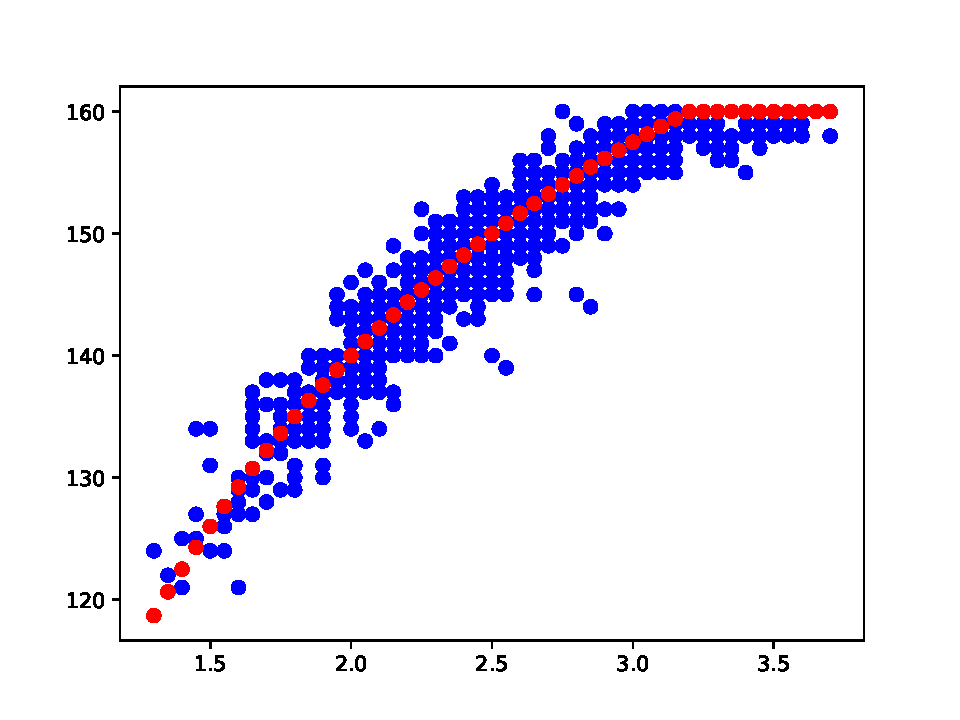
\includegraphics[width=0.48\textwidth]{./Figures/diff_1.pdf}}
  \subfigure[Average of 50 instances for each probability combination]{
    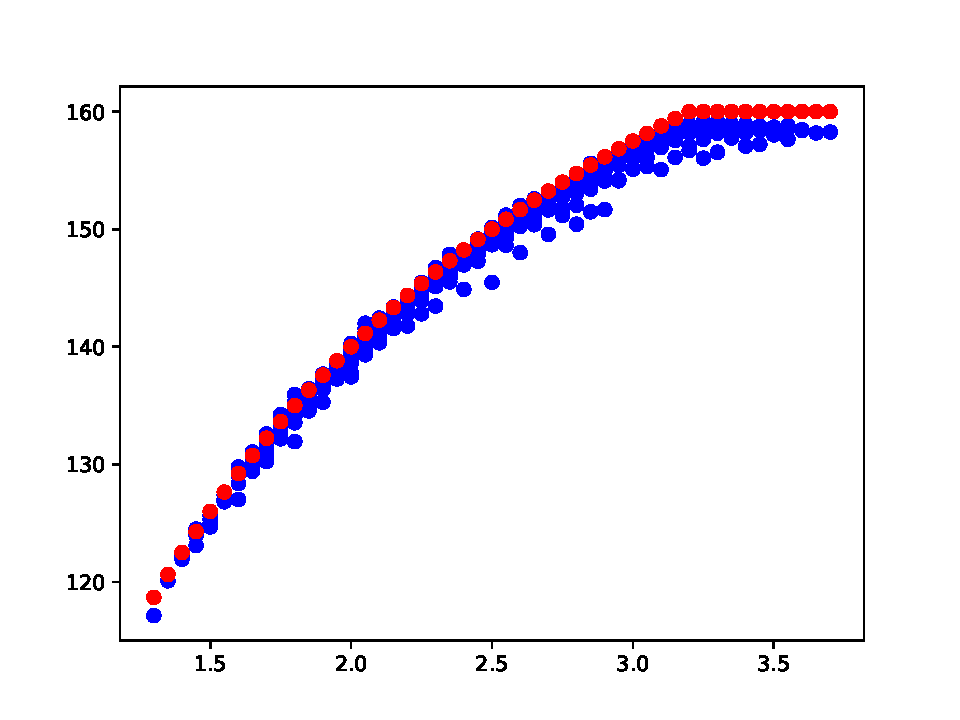
\includegraphics[width=0.48\textwidth]{./Figures/diff_2.pdf}}
  \caption{The number of people accepted versus $\gamma$}
\end{figure}


If the largest pattern is assigned to each row, the resulting occupancy rate is $\frac{16}{21}$. The maximum number of people that can be accepted is $210 * \frac{16}{21} = 160$, which is the upper bound on the number of people that can be accepted. The estimated number of people accepted is given by $\frac{\gamma}{\gamma+1} * 210$, as indicated by the red points in the figure.

However, we have also observed that some blue points in the figure are significantly far from the corresponding red points. For instance, when the probability combination is $[0.05, 0.05, 0.85, 0.05]$ (which corresponds to $\gamma = 2.9$), the demands may be such that they cannot be accommodated by constructing full patterns for every row. This does not satisfy our assumption and results in a large gap between the blue and red points in this case. For example, the demands could be $[4, 1, 45, 2]$ or $[2, 2, 47, 1]$.
% 改变 seat layout,  outlier 会消失。 
% 

\subsubsection{Results of Different Seat Layouts}
We compare two seat layouts with the same total number of seats. The first layout has rows with 17, 18, 19, 20, 21, 21, 22, 23, 24, and 25 seats, while the second layout has rows with 19, 20, 21, 21, 23, 24, 26, 17, 19, and 20 seats. Both layouts can accommodate a maximum of 164 people when each row corresponds to a largest pattern.

\begin{figure}[ht]
  \centering
  \subfigure[Average of 50 instances for step-size seat layout]{
    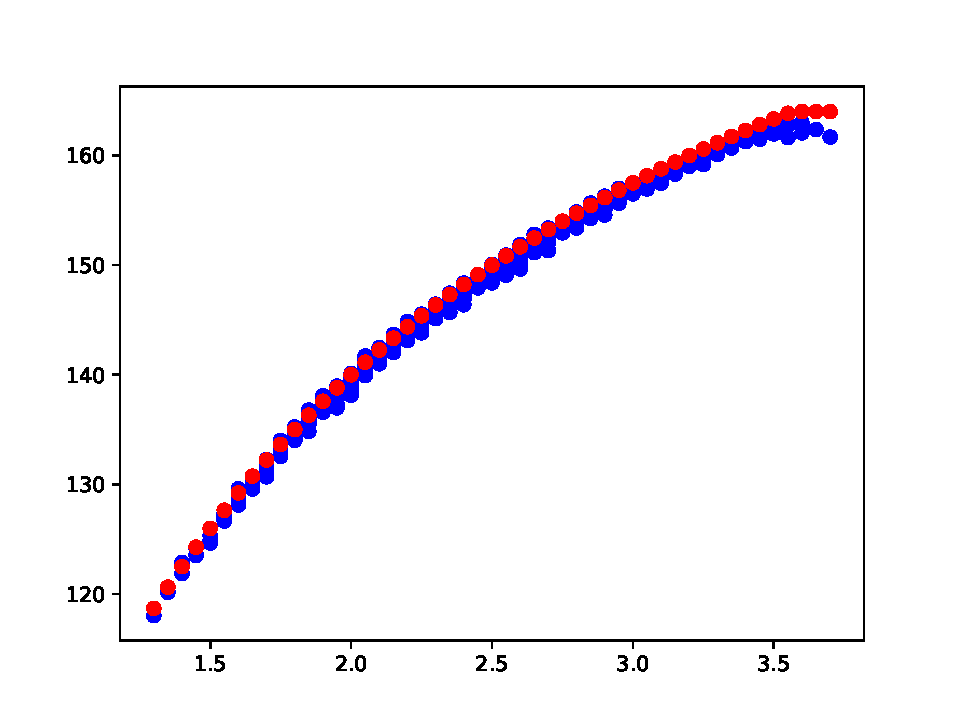
\includegraphics[width=0.48\textwidth]{./Figures/stepsize_seat.pdf}}
  \subfigure[Average of 50 instances for random seat layout]{
    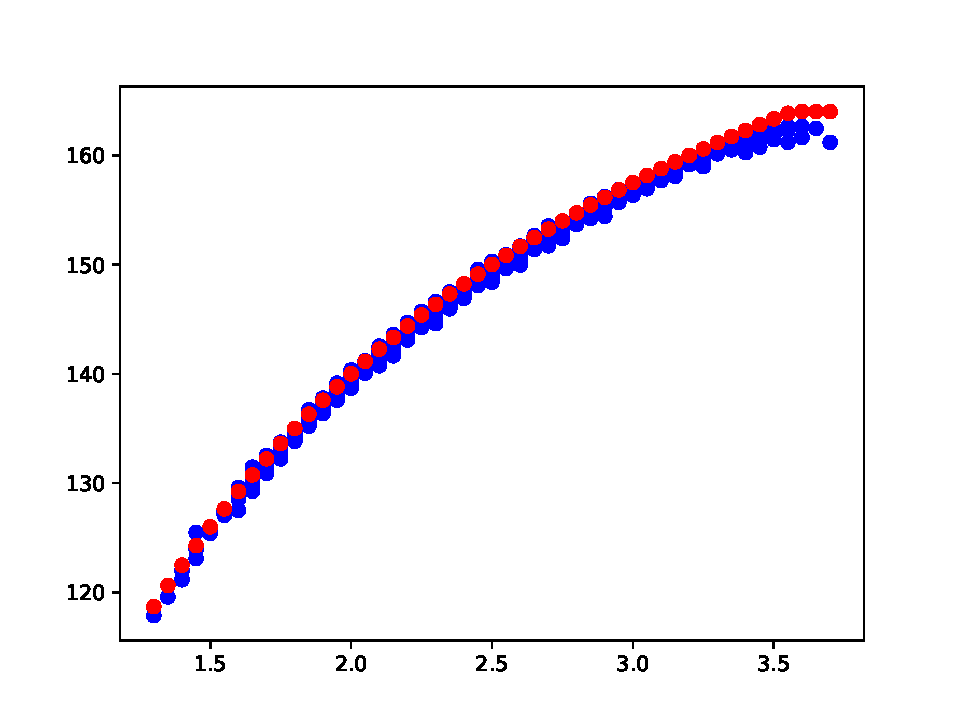
\includegraphics[width=0.48\textwidth]{./Figures/random_seat.pdf}}
  \caption{The number of people served versus $\gamma$}
\end{figure}

We can see that random seat layout will lead to a more accurate estimation, which means a random seat layout is likely to construct a full pattern so that to accept more people when facing the uncertain demands.


% When $p = [0.25, 0.25, 0.25, 0.25]$, $E(D) = 2.5 T$. Let $p_1*1 + p_2*2 + p_3*3 + p_4*4 = 2.5$, 
% Let $E(D) = 150, T = 50, 60, 75$. The number of seats: 200, 210, 225.

We can give the absolute difference between the blue point and red point for each probability combination as below.

\begin{table}[ht]
  \centering
  \caption{Difference Distribution}
  \begin{tabular}{|l|l|l|l|l|}
  \hline
  \# of instances & abs\_diff $\geq$ 1 & abs\_diff $\geq$ 2 & abs\_diff $\geq$ 3 & abs\_diff $\geq$ 4 \\
  \hline
  20 & 32.92 \% & 5.13 \% & 1.74\% & 0.51 \% \\
  50 & 22.46 \% & 4.31 \% & 1.54 \% & 0.31 \%  \\
  100 & 20.00 \% & 4.21 \% & 1.54 \% & 0.31 \% \\
  \hline
  \end{tabular}
\end{table}

\begin{figure}[ht]
  \centering
  \subfigure[Average of 50 instances for each probability combination]{
    \label{Fig1}
    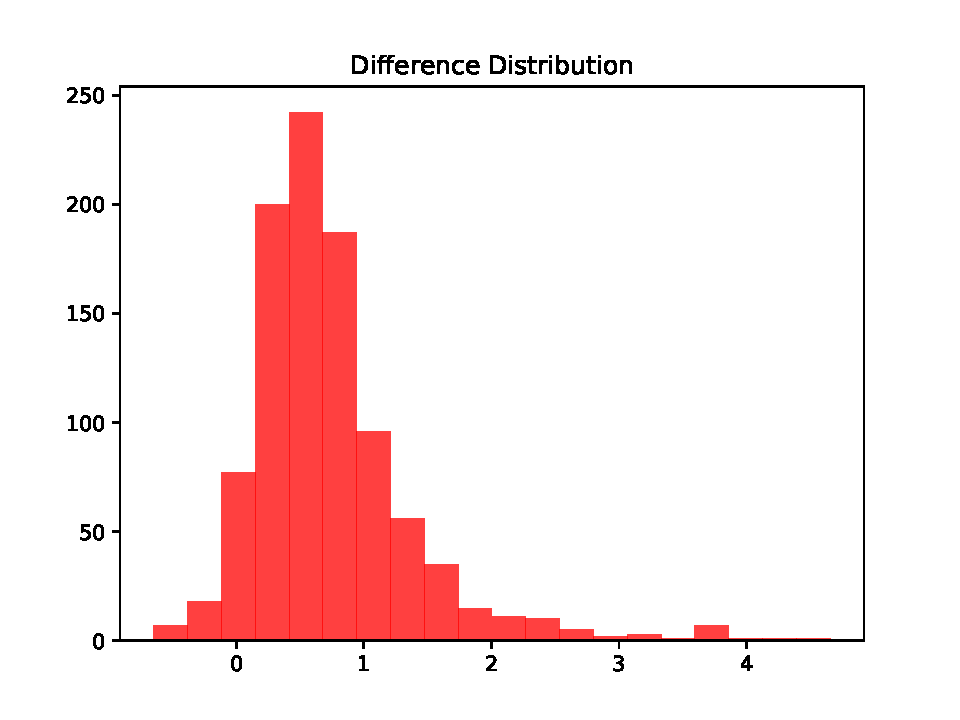
\includegraphics[width=0.48\textwidth]{./Figures/Figure_50.pdf}}
  \subfigure[Average of 100 instances for each probability combination]{
    \label{Fig2}
    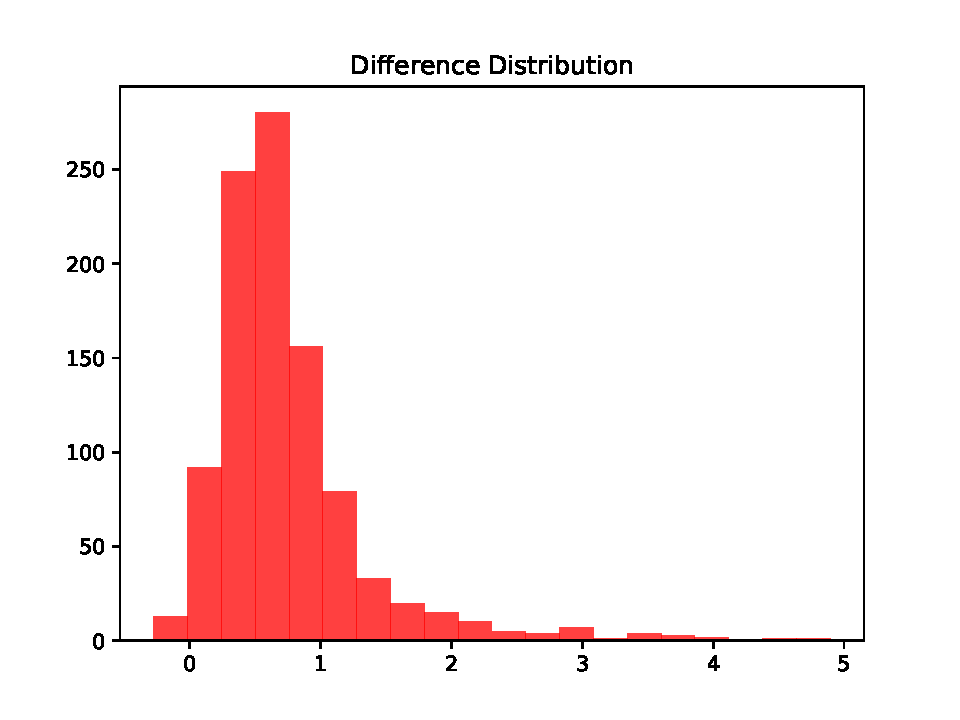
\includegraphics[width=0.48\textwidth]{./Figures/Figure_100.pdf}}
  \caption{The difference distribution}
  \label{Fig}
\end{figure}

The results show that we can estimate attendance rate based on $\gamma$ for most probability combinations. 

\subsection{Result of Different Demands}
% We then compare the number of people served under different values of $\gamma$.
In this subsection, we discuss the effect of the number of periods on the results of our experiments. Specifically, we consider two situations: $\gamma = 2.5$ and $\gamma = 1.9$.

When $\gamma = 2.5$, we set the parameters as follows: T = 10-100, step size = 1, expected number of periods = 60, expected number of demand (people) = 150, number of rows = 10, and number of seats per row = 21.

When $\gamma = 1.9$, we set the parameters as follows: T = 30-120, step size = 1, expected number of periods = 72, expected number of demand (people) = 137, number of rows = 10, and number of seats per row = 21.

For each $\gamma$, we give several probabilities in the table. The gap point represents the first period where the number of people without social distancing is larger than that with social distancing and the gap percentage is the corresponding percentage of total seats.


% We can find that the difference between the number of accepted people and the number of total people will increase with the period. 

\begin{table}[ht]
  \centering
  \caption{Gap points of different probabilities}
  \begin{tabular}{|l|l|l|l|}
  \hline
  $\gamma$  & probabilities & gap point & gap percentage \\
  \hline
  2.5  & [0.25,0.25,0.25,0.25] & 56 & 65.21 \\
  2.5  & [0.1,0.4,0.4,0.1] & 55 & 65.59 \\
  2.5  & [0.1, 0.5, 0.2, 0.2] & 55 & 65.45 \\
  2.5  & [0.2, 0.3, 0.3, 0.2] & 54 & 64.56 \\
  2.5  & [0.3, 0.2, 0.2, 0.3] & 55 & 65.51\\
  2.5  & [0.2, 0.4, 0.1, 0.3] & 55 & 65.41 \\
  1.9  & [0.4, 0.4, 0.1, 0.1] & 67 & 60.35 \\
  1.9  & [0.5, 0.2, 0.2, 0.1] & 67 & 58.9  \\
  1.9  & [0.3, 0.5, 0.2, 0]  &  68 & 61.7  \\
  1.9  & [0.6, 0.1, 0.1, 0.2] & 66 & 58.31 \\
  \hline
  \end{tabular}
\end{table}


We provide the results of our experiments for people accepted when applying social distance and not applying social distance over different periods. The different probabilities with the same $\gamma$ share the similar pattern of the figure, so we only provide one case to show the detailed figure.


\begin{figure}[h]
  \centering
  \subfigure[When $\gamma =2.5$]{
    \label{Fig.sub.1}
    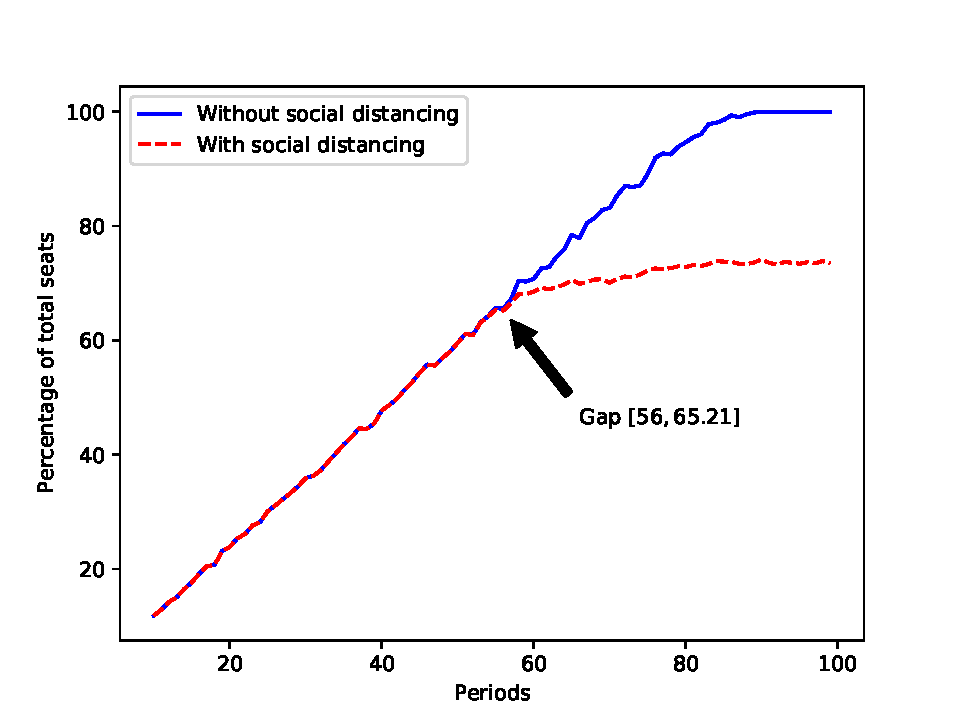
\includegraphics[width=0.48\textwidth]{./Figures/p1.pdf}}
  \subfigure[When $\gamma =1.9$]{
    \label{Fig.sub.2}
    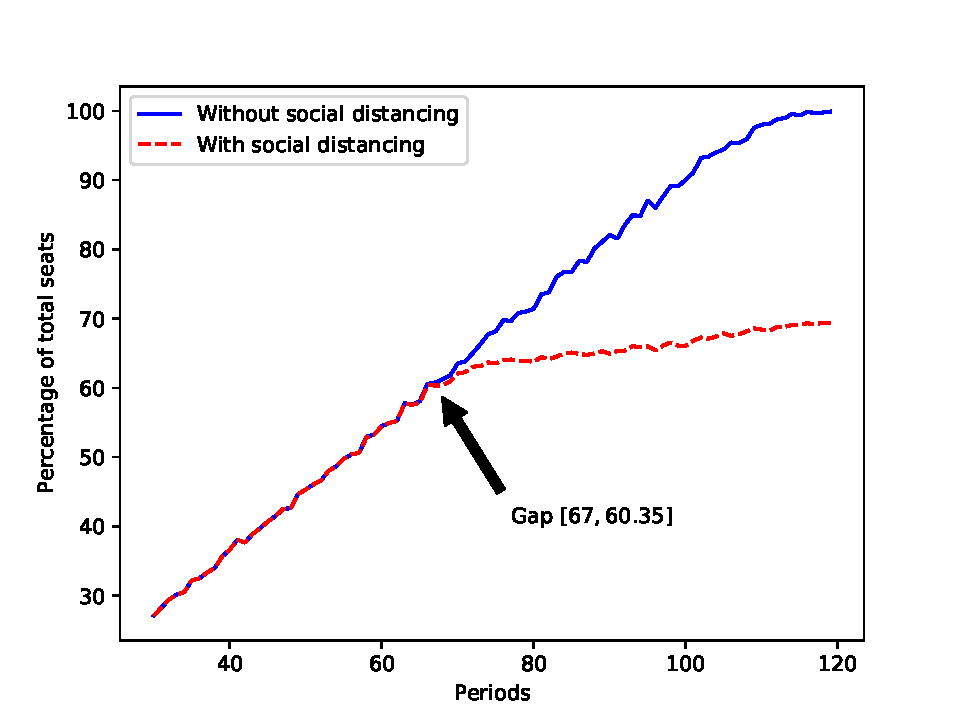
\includegraphics[width=0.48\textwidth]{./Figures/p2.pdf}}
  \caption{The number of people served versus periods}
  \label{Fig.lable}
\end{figure}


There are three stages, the first stage is when the capacity is sufficient. The measure of social distancing will not cause any effect. The gap is becoming larger as $T$ increases at the second stage. At the third stage, as $T$ continues to increase, the gap will converge when the capacity is limited.

We can estimate the attendance rate from $\frac{\gamma}{\gamma+1}*$ the number of seats. The number of periods will be $E(D)/\gamma$. Thus, the government can make the policy on how much attendance rate can be established.


\newpage

% \subsection{Group of Different Sizes}
% Let $\gamma$ be $2.5$ for groups of different sizes.

% Probability of group size of 3: $[0.1, 0.3, 0.6]$.

% Probability of group size of 5: $[0.3, 0.3, 0.1, 0.2, 0.1]$.

% \begin{figure}[h]
%   \centering
%   \subfigure[group size of 3]{
%     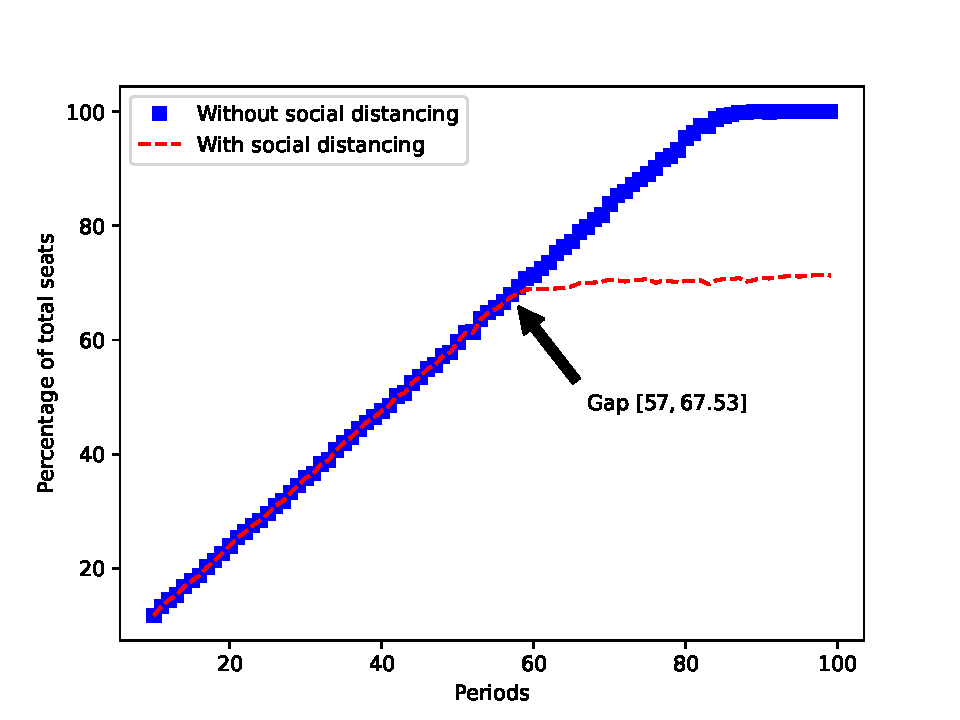
\includegraphics[width=0.48\textwidth]{./Figures/group3.pdf}}
%   \subfigure[group size of 5]{
%     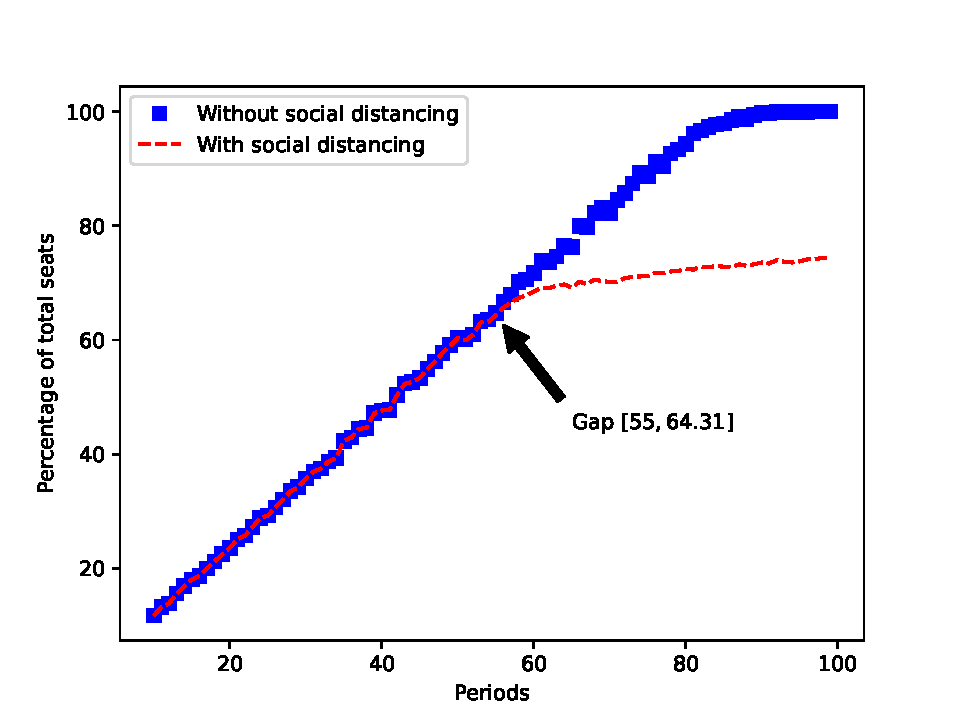
\includegraphics[width=0.48\textwidth]{./Figures/group5.pdf}}
%   \caption{The number of people served versus periods}
% \end{figure}

% \subsection{Measurement}

% Suppose a real scenario with a fixed sequence, $s^{r}$. Solving the following program can obtain the optimal value, $V_{s^{r}}$. (Offline)

% Then the difference is $V_{s^{r}} - \text{our result}$.

% WS(the value under wait-and-see policy with all possible scenarios)

% EVPI(Expected Value of Perfect Information) = WS - the value of deterministic equivalent form
